% ch12-systems.tex -- Processes and scheduling
\chapter{Processes and scheduling}
\label{ch:systems12}
\index{process}\index{context switch}\index{scheduler}\index{MLFQ}

Part IV starts here. Think of a single cook in a kitchen with ten
orders on the board. The cook cannot cook ten dishes at the same
instant, yet every customer feels served, because the cook keeps
stepping from one pot to the next and remembers exactly where each
dish stands. A computer does the same thing: a few cores serve
hundreds of programs by switching between them so quickly that each
program feels like it owns the machine. The operating system is the
cook's habit of keeping notes. This chapter builds the two ideas
behind that habit. The first is the \emph{process}, the bundle of
notes about one running program. The second is the \emph{scheduler},
the rule that decides whose turn it is. We also measure what a
switch costs on a real machine instead of quoting a number from a
book.

\begin{wins}[What you will be able to do]
After this chapter you can write a C program that starts another
program and collects its exit status without leaking a zombie (a
finished process nobody has collected yet). You can wire a
three-stage pipeline by hand, the way a shell does. You can measure
what a context switch costs on your own machine and explain why the
number changes when you pin the program to one CPU. And you can take
any list of jobs with arrival times and lengths and compute average
turnaround and response time under five scheduling rules, by hand
and with the chapter's simulator.
\end{wins}

\begin{rulebox}[Before you start]
Three earlier ideas carry this chapter, so here is a quick recap.
\emph{Traps} (Book~7 ch.~\ref{ch:systems08}): when a timer fires or a
program asks the kernel for something, the CPU saves where it was
and jumps to a kernel routine; a context switch rides on exactly
that path. \emph{Virtual memory} (ch.~\ref{ch:systems11}): every
process sees its own private address space, which the hardware maps
to real memory through a page table. After a \texttt{fork} the two
processes share pages \emph{copy-on-write} (COW): a page is copied
only at the moment someone writes to it, like two people reading one
newspaper until one of them wants to scribble on it. \emph{State
machines} (Book~5 ch.~10, sequential circuits and state machines): a
thing with a few named states that changes state on events. A process
is exactly that, as you will see. If you want to count time units the
way the simulator does, Book~1 ch.~1 (the contest machine and the
cost model) is where counting operations began.

\emph{A short C refresher, enough for this chapter.} A program is
compiled with \texttt{gcc file.c -o file} and started with
\texttt{./file}. \texttt{pid\_t} is an integer type that holds a
process id. \texttt{fork()} returns $-1$ if it failed, $0$ in the new
child, and the child's pid in the parent; the same line of code runs
twice, once in each process. \texttt{waitpid(p, \&st, 0)} passes the
\emph{address} of the integer \texttt{st} (the \texttt{\&} means
``address of'') so the function can write the child's status into it
for you; \texttt{WEXITSTATUS(st)} then reads the exit code out.
\texttt{char *argv[] = \{"echo", "hi", NULL\}} is an array of strings
ended by \texttt{NULL}, which is the form \texttt{exec} expects.

\emph{Where the numbers come from.} Every command here ran on a
Linux x86\_64 container (4 vCPU Intel Xeon at 2.8\,GHz, kernel 6.18,
gcc 13). Numbers marked \emph{Mac} were measured earlier on the
author's laptop and are kept as they were; the two machines are never
mixed in one comparison.
\end{rulebox}

\begin{principle}[Think like this]
Whenever a system seems to do two things at once, ask: what is the
\emph{saved note} that lets it stop and resume, and who decides when
to switch? Almost every idea in this chapter is an answer to one of
those two questions.
\end{principle}

\section{What a process is}
\label{sec:proc12}

A process is a running program's whole state bundled: an address
space (ch11's private map), a register set saved somewhere, open
files, and a kernel bookkeeping entry. The CPU sees none of it ---
it just executes instructions and takes traps. The OS's job is to
suspend that state, park it, and restore a different one.

\begin{principle}[Concept: a process is a program plus its bookmark]
A recipe in a cookbook is a \emph{program}: it just sits there. A cook
halfway through that recipe, with the pot on the stove and a finger
on step 4, is a \emph{process}. Two cooks following the same recipe
are two processes of one program. Everything the OS must write down
to pause one cook and later resume exactly where they were (the
registers, the memory map, the open files) is the bookmark. Without
the bookmark, switching would lose work; with it, switching is only
a matter of copying a few values.
\end{principle}

Figure~\ref{fig:states12} is the whole life of a process in three
states. \emph{Running} means a core is executing it right now.
\emph{Ready} means it could run but is waiting for a core.
\emph{Blocked} means it is waiting for something slow, such as a
disk read, and would waste a core if given one. When a process
finishes it becomes a zombie until its parent collects the result,
a detail we meet with real output below.

\begin{figure}[htbp]
\centering
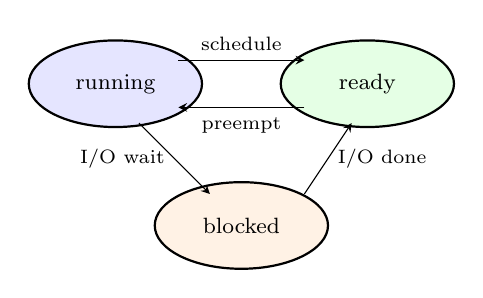
\begin{tikzpicture}[font=\footnotesize, >=stealth, x=1cm, y=1cm]
  \draw[thick,fill=blue!10] (0,2.6) ellipse (1.1 and 0.55);
  \node at (0,2.6) {running};
  \draw[thick,fill=green!10] (3.2,2.6) ellipse (1.1 and 0.55);
  \node at (3.2,2.6) {ready};
  \draw[thick,fill=orange!10] (1.6,0.8) ellipse (1.1 and 0.55);
  \node at (1.6,0.8) {blocked};
  \draw[->] (0.8,2.9) -- (2.4,2.9) node[midway,above]{\scriptsize schedule};
  \draw[->] (2.4,2.3) -- (0.8,2.3) node[midway,below]{\scriptsize preempt};
  \draw[->] (0.3,2.1) -- (1.2,1.2) node[midway,left]{\scriptsize I/O wait};
  \draw[->] (2.4,1.2) -- (3.0,2.1) node[midway,right]{\scriptsize I/O done};
\end{tikzpicture}
\caption{The three-state life of a process. The scheduler moves a
process between ready and running; the I/O system moves it between
running and blocked. Everything else --- priorities, queues,
timeslices --- is policy on top of this machine.}
\label{fig:states12}
\end{figure}


\section{fork, exec, wait --- the correct version}
\label{sec:few12}

Why does UNIX start a new program in two steps instead of one?
Because the gap between the steps is useful. After \texttt{fork}
and before \texttt{exec}, the child can still rearrange its own
plumbing (redirect output to a file, close a descriptor, change
directory) using ordinary code, and then become the new program.
A single ``spawn'' call would need a flag for every such wish.
UNIX's recipe is two calls, not one: \texttt{fork} duplicates the
process (child gets a copy of everything --- COW, ch11, makes it
nearly free), \texttt{exec} replaces the copy's program image with a
new one. A shell pipeline \texttt{ps | grep x | wc} costs three
forks and three execs.

\begin{lstlisting}[language=C,caption={The three mistakes almost
everyone makes, avoided: check \texttt{fork}'s error path, handle
\texttt{exec} failure with \texttt{\_exit}, and wait on
\emph{status}, not just completion.}]
pid_t p = fork();
if (p < 0) { perror("fork"); return 1; }   // fork CAN fail
if (p == 0) {
    execl("/bin/echo", "echo", "hi", NULL);
    _exit(127);                            // exec failed: exit, not return
}
int st; pid_t w = waitpid(p, &st, 0);      // harvest the status
\end{lstlisting}

The real output of the chapter's fork demo
(\texttt{ch12\_fork\_demo.c}, Linux x86\_64 container): the exec'd
echo printed \texttt{hello from exec'd child}, then the parent
printed its clean \texttt{waitpid} line (\texttt{status=0}), and the
child's exit status arrives intact.

\begin{lstlisting}[basicstyle=\ttfamily\scriptsize,caption={Real output
of \texttt{ch12\_fork\_demo} (pids differ on every run).}]
parent 4790 starting
  child 4792 exec'ing /bin/echo
  hello from exec'd child
parent: child 4792 exited, status=0
\end{lstlisting}

One detail in that source is easy to miss: it calls
\texttt{fflush(stdout)} before \texttt{fork} and before \texttt{exec}.
When standard output is a pipe or file, C buffers it in user memory.
A forked child inherits a copy of the unflushed buffer, and
\texttt{exec} then throws the buffer away. Our first capture, run
through a pipe \emph{without} those two calls, printed the parent's
line late and lost the child's ``exec'ing'' line entirely.

\begin{example}[Fork returns twice, and the memory is a copy]
\emph{What goes wrong first.} A beginner writes \texttt{x += 1} in
the child and expects the parent to see 101, as two threads would. It
does not, because the two processes do not share \texttt{x}.
\texttt{ch12\_cow.c} shows it:

\begin{lstlisting}[language=C,basicstyle=\ttfamily\scriptsize,caption={\texttt{fork}
returns once in each process; the child's write stays private.}]
int x = 100;
pid_t p = fork();
if (p == 0) { x += 1; printf("child : fork returned %d, x=%d, &x=%p\n", (int)p, x, (void*)&x); return 0; }
waitpid(p, NULL, 0);
printf("parent: fork returned child pid > 0: %s, x=%d, &x=%p\n", p > 0 ? "yes" : "no", x, (void*)&x);
\end{lstlisting}
\begin{lstlisting}[basicstyle=\ttfamily\scriptsize,caption={Real output. The
address is the same, the value is not (the address changes between
runs because of ASLR, address-space randomisation).}]
child : fork returned 0, x=101, &x=0x55e749afa010
parent: fork returned child pid > 0: yes, x=100, &x=0x55e749afa010
\end{lstlisting}
Both processes print the \emph{same virtual address} and different
values. Each has its own page table (ch.~\ref{ch:systems11}); after
the fork both map the page read-only and shared, and the child's
write triggers the COW fault that gives it a private copy. The
return value is the only way the two copies of the code tell
themselves apart.
\end{example}

\begin{example}[Forgetting to wait: the zombie]
\emph{What goes wrong first.} A parent forks a child that exits at
once and never calls \texttt{wait}. The child is finished, yet its
kernel entry cannot go away: the exit status (here 7) must stay
available in case the parent asks. A finished-but-unreaped process is
a \emph{zombie}. \texttt{ch12\_zombie.c} reads the state letter from
\texttt{/proc/PID/stat} before and after \texttt{waitpid}:

\begin{lstlisting}[language=C,basicstyle=\ttfamily\scriptsize,caption={The parent
looks at its child's state, reaps it, and looks again.}]
pid_t p = fork();
if (p == 0) _exit(7);                    // child: exit at once, status 7
usleep(100000);                          // let it finish
printf("before waitpid: child state = %c\n", state_of(p));
int st; waitpid(p, &st, 0);
printf("waitpid returned: exit status = %d\n", WEXITSTATUS(st));
printf("after  waitpid: child state = %c\n", state_of(p));
\end{lstlisting}
\begin{lstlisting}[basicstyle=\ttfamily\scriptsize,caption={Real output
(\texttt{Z} is zombie; \texttt{-} means \texttt{/proc} has no such pid).}]
before waitpid: child state = Z
waitpid returned: exit status = 7
after  waitpid: child state = -
\end{lstlisting}
A zombie uses no CPU and almost no memory, but it holds a
process-table slot, and a parent that leaks thousands of them can run
the system out of pids. You cannot \texttt{kill} a zombie: it is
already dead. The only cure is for the parent to call \texttt{wait}
(or to exit, after which the init process adopts and reaps the
orphans).
\end{example}

\begin{example}[A shell pipeline built by hand]
A shell turns \texttt{echo "hello systems" | tr a-z A-Z | wc -c}
into three forks, two pipes and three execs. A \emph{pipe} is a
kernel buffer with a read end and a write end, each a file
descriptor. \texttt{dup2(fd, 0)} makes descriptor 0 (standard input)
refer to the same thing as \texttt{fd}; that is how the pipe end
becomes the program's stdin without the program knowing.
\texttt{ch12\_pipeline.c} runs the sequence:

\begin{lstlisting}[language=C,basicstyle=\ttfamily\scriptsize,caption={The wiring in
\texttt{ch12\_pipeline.c} (the helper \texttt{spawn} forks, calls
\texttt{dup2}, closes every pipe end, then \texttt{execvp}s).}]
int p1[2], p2[2]; pipe(p1); pipe(p2);          // p[0] = read end, p[1] = write end
spawn(echo, 0,     p1[1], ...);                // echo: stdout -> p1 write end
spawn(tr,   p1[0], p2[1], ...);                // tr:   stdin <- p1, stdout -> p2
spawn(wc,   p2[0], 1,     ...);                // wc:   stdin <- p2, stdout stays the terminal
close(p1[0]); close(p1[1]); close(p2[0]); close(p2[1]);   // the parent closes ALL four
while (wait(&st) > 0) n++;
\end{lstlisting}
\begin{lstlisting}[basicstyle=\ttfamily\scriptsize,caption={Real output. \texttt{wc -c}
counts the 13 letters of ``HELLO SYSTEMS'' plus the newline.}]
14
parent reaped 3 children
\end{lstlisting}
\emph{What goes wrong first.} Skip the parent's four \texttt{close}
calls and the program hangs. A reader sees end-of-file on a pipe only
when \emph{every} copy of the write end is closed, and the parent
still holds one, so \texttt{tr} waits forever for more input. We
checked this by compiling the same file with a build flag that
omitted those closes and running it under \texttt{timeout 2}: it was
killed (exit status 124) instead of printing.
\end{example}

\section{The context switch, step by step}
\label{sec:ctx12}

\begin{figure}[htbp]
\centering
\begin{tabular}{ll}
\toprule
step & what the kernel does \\
\midrule
1 & trap arrives (timer tick, syscall, fault) \\
2 & save $P_1$'s registers on $P_1$'s kernel stack \\
3 & \texttt{swtch}: swap stack pointer to $P_2$'s context \\
4 & restore $P_2$'s registers from its stack \\
5 & return-from-trap into $P_2$'s userspace \\
\bottomrule
\end{tabular}
\caption{A context switch is just a stack-pointer swap between two
pre-staged register saves --- the same trap machinery from ch8,
aimed at a different address space. Cost on this machine:
$\approx$3\,\textmu s measured.}
\label{fig:ctxsw12}
\end{figure}


Nothing new is invented here: a context switch reuses ch8's trap
path exactly --- registers get saved, the kernel swaps which saved
set to restore, and the machine returns into a different address
space. The only fresh piece is \texttt{swtch}, the stack-pointer
swap.

\begin{example}[The 3\,\textmu s truth, measured]
\texttt{ch12\_ctx\_switch.c} ping-pongs a byte through pipes; each
round trip costs two switches. On the Mac: \textbf{2.93\,\textmu s
per switch} at one pair, 3.7 at two, 3.1 at four. The flat scaling
is the honest confound --- extra pairs spread across cores rather
than queueing --- and the number is the real price of the illusion:
$\approx$300 switches before one millisecond is spent.
\end{example}

\begin{figure}[htbp]
\centering
\begin{tabular}{lr}
\toprule
configuration & measured \textmu s/switch \\
\midrule
\multicolumn{2}{l}{\emph{Mac (author's laptop)}} \\
1 pipe pair   & 2.93 \\
2 pairs       & 3.71 \\
4 pairs       & 3.14 \\
\midrule
\multicolumn{2}{l}{\emph{Linux x86\_64 container, median of 3}} \\
1 pair, unpinned & 19.58 \\
2 pairs, unpinned & 18.01 \\
4 pairs, unpinned & 17.95 \\
1 pair, pinned (\texttt{taskset -c 0}) & 2.06 \\
2 pairs, pinned & 2.70 \\
4 pairs, pinned & 3.35 \\
\bottomrule
\end{tabular}
\caption{Real \texttt{ch12\_ctx\_switch.c} output. On the Mac,
$\approx$3\,\textmu s per switch, with flat scaling because extra
pairs spread over cores. On the Linux container, unpinned runs cost
$\approx$18--20\,\textmu s (cross-core wake-ups in a virtual machine)
and pinned runs 2--3.4\,\textmu s. The two machines are different
experiments and are not compared digit for digit.}
\label{fig:ctxcost12}
\end{figure}


\begin{example}[Pinned versus unpinned: the same program, a 7$\times$ different answer]
\emph{What goes wrong first.} We built the pipe ping-pong, ran it,
and on the Linux container it reported about 20\,\textmu s per
switch, nearly ten times the Mac figure above. The program had not
changed. What changed is where the two processes ran. When the
parent writes a byte and sleeps in \texttt{read}, the kernel has to
wake the child. If the child lives on another core, waking it means
sending that core an inter-processor interrupt, and in a virtual
machine that signal is expensive. If both processes are \emph{pinned}
to one core (told to run only there), the ``wake-up'' is just the
next thing the same core does.

\begin{lstlisting}[basicstyle=\ttfamily\scriptsize,caption={Real runs on the
Linux x86\_64 container, three each; the \texttt{taskset -c 0} prefix pins the
program and its children to CPU 0.}]
$ ./ctx_switch 1                    $ taskset -c 0 ./ctx_switch 1
pairs=1  19.94 us per ctx switch    pairs=1  2.13 us per ctx switch
pairs=1  19.58 us per ctx switch    pairs=1  2.06 us per ctx switch
pairs=1  18.23 us per ctx switch    pairs=1  1.98 us per ctx switch
\end{lstlisting}

The unpinned median is 19.6\,\textmu s and the pinned median 2.06\,\textmu s,
a ratio of $19.6/2.06\approx 9.5$. Across all our runs unpinned
values ranged from 6.8 to 22.8\,\textmu s (the machine is shared, so
they wander), while pinned values stayed between 2.0 and 3.7. The
lesson is a habit worth keeping: before you trust a timing, ask which
physical resources the two sides of the test were using.
\end{example}

\begin{principle}[Think like this]
A measurement answers one specific question. ``How long is a context
switch?'' hides two questions: the cost of the kernel swapping
state, and the cost of waking a process on another core. Pinning
removes the second so that you are measuring the first.
\end{principle}

\begin{checkpoint}
Why is the context-switch number not simply ``instructions
executed''? Because the pipeline cost dominates: every switch
invalidates the cache-warm state, the TLB entries, the branch
predictor --- the machine runs cold for thousands of cycles after.
\end{checkpoint}

\section{Scheduling: five policies, measured on one job set}
\label{sec:sched12}

Why does a scheduler need a policy at all? Because whenever more
jobs are ready than there are cores, someone must wait, and the order
of waiting changes how the whole system feels. Picture a supermarket
with one till. If a person with a full trolley is first in line,
everyone behind them with one carton of milk waits a long time;
letting the milk-buyers go first costs the trolley person very
little. That intuition is what the policies below try to capture, and
we need two precise words to compare them. \emph{Turnaround time} is
finish time minus arrival time: how long the job spent in the system.
\emph{Response time} is first-run time minus arrival time: how long
before the job first got any attention.

The job set: A(100), B(30), C(10), D(60) time units, arriving at
0, 10, 20, 30. The chapter's simulator runs five rules on it. FIFO
(first in, first out) runs jobs to completion in arrival order. SJF
(shortest job first) picks the shortest waiting job whenever the
core is free, but never interrupts a running job. STCF (shortest
time to completion first) is SJF that \emph{may} interrupt: when a
new job arrives with less work left than the running one, it takes
over. RR (round robin) gives each ready job a fixed slice, here 10
units, in turn. MLFQ (multi-level feedback queue) is described
below.

\begin{figure}[htbp]
\centering
\begin{tikzpicture}[font=\footnotesize, x=0.057cm, y=1cm]
  \tikzset{blk/.style={draw=ink, thin, minimum height=0.7cm, inner sep=0pt, anchor=south west}}
  \definecolor{jobA}{HTML}{DCE3F0}\definecolor{jobB}{HTML}{DDEBE2}
  \definecolor{jobC}{HTML}{F1E3CF}\definecolor{jobD}{HTML}{E4E4E4}
  % FIFO row
  \node[anchor=east] at (-3,1.9) {FIFO};
  \foreach \s/\e/\j in {0/100/A,100/130/B,130/140/C,140/200/D}{
    \node[blk, fill=job\j, minimum width={(\e-\s)*0.057cm}] at (\s,1.55) {\j};}
  % STCF row
  \node[anchor=east] at (-3,0.4) {STCF};
  \foreach \s/\e/\j in {0/10/A,10/20/B,20/30/C,30/50/B,50/110/D,110/200/A}{
    \node[blk, fill=job\j, minimum width={(\e-\s)*0.057cm}] at (\s,0.05) {\j};}
  % time axis
  \draw[->] (0,-0.3) -- (206,-0.3) node[right]{\scriptsize time};
  \foreach \t in {0,10,20,30,50,100,110,130,140,200}{
    \draw (\t,-0.22) -- (\t,-0.38); \node[below, font=\tiny] at (\t,-0.38) {\t};}
\end{tikzpicture}
\caption{The same four jobs (A\,100, B\,30, C\,10, D\,60; arriving at
0, 10, 20, 30) under FIFO and STCF. FIFO runs each job to completion
in arrival order, so B, C and D all wait behind A. STCF switches at
every arrival and finish (five switches) and runs A last. Both rows
are the schedules behind the turnaround numbers in
Figure~\ref{fig:schedcmp12}.}
\label{fig:gantt12}
\end{figure}


\begin{figure}[htbp]
\centering
\begin{tabular}{lrrr}
\toprule
policy & avg turnaround & avg response & order \\
\midrule
FIFO & 127.5 & 77.5 & ABCD \\
SJF  & 122.5 & 72.5 & ACBD \\
STCF & 82.5  & 5.0  & ABCD \\
RR (slice 10) & 107.5 & 7.5 & --- \\
MLFQ (10/20/40) & 97.5 & 0.0 & --- \\
\bottomrule
\end{tabular}
\caption{Real \texttt{sched\_sim.py} output on the chapter's job set
(A:100, B:30, C:10, D:60 time units): STCF's preemption buys a
35\% turnaround win and a 15$\times$ response win --- the
interactivity argument, measured not asserted. RR and MLFQ rows
come from the extended simulator in this chapter's listing (same
job set; MLFQ has three levels with slices 10, 20, 40 and a boost
every 100 units).}
\label{fig:schedcmp12}
\end{figure}


\begin{example}[What the numbers argue]
FIFO's 127.5 turnaround is the convoy problem: B, C, D all wait
behind 100-unit A. STCF's preemption drops response time to 5.0 ---
interactive jobs feel instant. SJF without preemption buys almost
nothing here. The policy debate is numerical, not aesthetic.
\end{example}

\begin{lstlisting}[basicstyle=\ttfamily\scriptsize,caption={Real output of
\texttt{python3 ch12\_sched\_sim.py}. The \texttt{switches} column
counts how many times the core changed from one job to another.}]
arrivals 0,10,20,30  (A=100 B=30 C=10 D=60)
policy turnaround  response switches  first-run/slice order
fifo        127.5      77.5        3  ABCD
sjf         122.5      72.5        3  ACBD
stcf         82.5       5.0        5  ABCBDA
rr          107.5       7.5       17  ABACBDABDADADADADA
mlfq         97.5       0.0        9  ABCDABDADA

all arrive at t=0
policy turnaround  response switches  first-run/slice order
fifo        142.5      92.5        3  ABCD
sjf          87.5      37.5        3  CBDA
stcf         87.5      37.5        3  CBDA
rr          120.0      15.0       16  ABCDABDABDADADADA
mlfq        112.5      15.0        9  ABCDABDADA
\end{lstlisting}

\begin{example}[Round robin by hand, then check the simulator]
\emph{Setup.} All four jobs present at time 0, slice 10, order
A, B, C, D. Walk the cycles. Cycle 1 runs A, B, C, D for 10 each
(time 0--40), and C, which needed only 10, finishes at 30. Cycle 2
runs A, B, D (40--70); cycle 3 runs A, B, D (70--100) and B, having
now had 30, finishes at \emph{its} slot ending at 90. At time 100
D has had three slices (30 of its 60 units) and A has had three too
(30 of 100), so they alternate A, D, A, D, A, D until D finishes at
160, and then A runs alone until 200. Turnarounds (arrival is 0, so turnaround
equals finish): C\,=\,30, B\,=\,90, D\,=\,160, A\,=\,200, so the average is
$(30+90+160+200)/4=120$, and the simulator's second table agrees
(\texttt{rr 120.0}). Notice what RR bought: response time 15 instead
of FIFO's 92.5, at the price of 16 switches instead of 3. SJF, which
never interrupts, reaches turnaround 87.5 with only 3 switches,
because here all jobs are known and equal arrival makes ``shortest
first'' exactly optimal for turnaround. The best policy depends on
which of the two numbers you care about.
\end{example}

\begin{example}[The convoy depends on who arrives first]
Compare the two tables. With staggered arrivals SJF scored 122.5,
barely better than FIFO's 127.5, because the long job A was already
running when the short ones arrived and SJF will not interrupt it.
With every job present at time 0, SJF scores 87.5, a drop of 35,
while FIFO gets \emph{worse} (142.5) since its order is still
A, B, C, D. Verify one entry by hand: SJF at $t=0$ runs C first
(finish 10), then B (40), then D (100), then A (200), so
$(10+40+100+200)/4=87.5$. A single policy's score is a property of
the policy \emph{and} the workload together.
\end{example}

\begin{figure}[htbp]
\centering
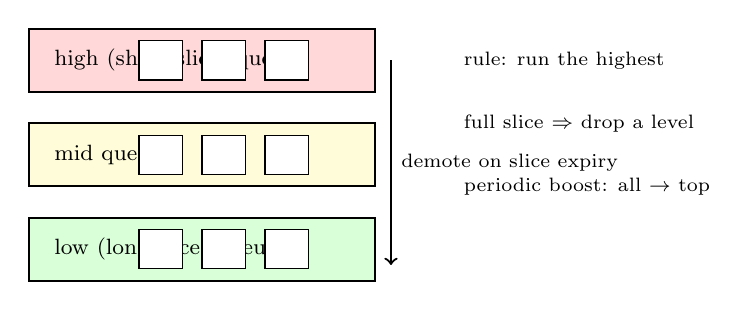
\begin{tikzpicture}[font=\footnotesize, x=1cm, y=1cm]
  \foreach \y/\pri/\fill in {3.4/{high (short slice)}/red!15,
                             2.2/{mid}/yellow!15,
                             1.0/{low (long slice)}/green!15} {
    \draw[thick,fill=\fill] (0,\y) rectangle (4.4,\y+0.8);
    \node[anchor=west] at (0.2,\y+0.4) {\pri\ queue};
    \foreach \x in {1.4,2.2,3.0} {
      \draw[fill=white] (\x,\y+0.15) rectangle (\x+0.55,\y+0.65); }
  }
  \draw[->,thick] (4.6,3.8) -- (4.6,1.2) node[midway,right]
    {\scriptsize demote on slice expiry};
  \node[anchor=west] at (5.4,3.8) {\scriptsize rule: run the highest};
  \node[anchor=west] at (5.4,3.0) {\scriptsize full slice $\Rightarrow$ drop a level};
  \node[anchor=west] at (5.4,2.2) {\scriptsize periodic boost: all $\to$ top};
\end{tikzpicture}
\caption{MLFQ without code: short jobs naturally fall to the bottom
(they finish before being demoted); long jobs sink and get long
slices; a periodic priority boost stops starvation. The policy
approximates STCF without knowing job lengths.}
\label{fig:mlfq12}
\end{figure}


MLFQ stands for multi-level feedback queue. Its problem: the
scheduler almost never knows how long a job will run, so STCF's
``shortest first'' cannot be applied directly. Its trick is to watch
instead of ask:
jobs that use their full slice sink to longer-slice queues (they
look like long jobs); interactive jobs stay high because they block
on I/O before the slice ends (they look short). A
periodic boost prevents starvation. Real schedulers (Linux's
CFS uses different math for the same ends) all answer the same
tension: turnaround vs.\ response.

\section{The few dozen lines that actually do it}
\label{sec:xv6_12}

\begin{figure}[htbp]
\centering
\begin{tabular}{p{0.9\linewidth}}
\toprule
Guided read --- xv6 \texttt{proc.c} \\
\midrule
\texttt{swtch.S}: 14 instructions that save callee-saved registers,
swap \texttt{sp}, restore the other side. The whole of a context
switch is literally those 14 lines --- ch8's trap path plus this.
\texttt{scheduler()}: a 6-line loop --- pick first RUNNABLE, switch
to it, repeat. The OS's most famous 20 lines do everything this
chapter's sim does, with real registers instead of arrays. \\
\bottomrule
\end{tabular}
\caption{The read-the-source payoff: xv6's context switch and
scheduler fit in about twenty lines between them. The policy
chapter's machinery is this small on a real OS.}
\label{fig:xv6_12}
\end{figure}


\section{Common mistakes}
\label{sec:mistakes12}
\begin{itemize}
\item \textbf{Skipping \texttt{fork}'s error path.} Fork bombs
      apart, resource limits make fork fail; an unchecked
      \texttt{fork()} becomes a crash or a zombie.
\item \textbf{\texttt{return} after a failed \texttt{exec}.} The
      child falls back into the parent's code --- use
      \texttt{\_exit} or \texttt{perror}+\texttt{\_exit}.
\item \textbf{\texttt{wait} only at program end.} Unreaped children
      zombie: harvest statuses as they exit.
\item \textbf{Treating ctx-switch cost as free.} 3\,\textmu s
      $\times$ thousands/sec is real time; thread pools exist
      because the number isn't zero.
\item \textbf{Forgetting to flush stdio before \texttt{fork}.} The
      child gets a copy of the unflushed buffer, so text can appear
      twice, late, or (after \texttt{exec}) not at all.
\item \textbf{Closing only some pipe ends.} A reader sees end-of-file
      only when every copy of the write end is closed, the parent's
      included; otherwise the pipeline hangs.
\item \textbf{Timing a switch without saying where the processes
      ran.} Pinned and unpinned runs differed by $9\times$ here.
\item \textbf{Optimising turnaround when you meant response.} STCF
      wins both on our set, but SJF's non-preemptive gain is nearly
      zero --- measure the metric you actually care about.
\end{itemize}

\section{Summary}
\label{sec:summary12}
\begin{tabularx}{\linewidth}{@{}l X@{}}
\toprule
\textbf{Piece} & \textbf{Verified version} \\
\midrule
process   & address space + saved state + kernel entry \\
fork/exec & duplicate then replace; COW makes fork O(1)-ish \\
ctx switch & trap + stack swap; $\approx$3\,\textmu s (Mac), 2.1\,\textmu s pinned / 19.6\,\textmu s unpinned (Linux container) \\
FIFO/SJF/STCF & 127.5 / 122.5 / 82.5 turnaround on real sim \\
RR (slice 10) & 107.5 turnaround, 7.5 response, 17 switches \\
MLFQ      & 97.5 turnaround, 0.0 response, 9 switches; needs no job lengths \\
zombie    & exited, status kept until the parent waits \\
xv6       & the real mechanism: 29 instructions of \texttt{swtch} plus a $\sim$20-line loop \\
\bottomrule
\end{tabularx}

\section*{Further reading}
\label{sec:further12}
\begin{itemize}
\item Arpaci-Dusseau \& Arpaci-Dusseau, OSTEP ch4--11 (the sim
      homework this chapter follows):
      \url{https://pages.cs.wisc.edu/~remzi/OSTEP/}
\item xv6 source, \texttt{proc.c}, \texttt{swtch.S}:
      \url{https://github.com/mit-pdos/xv6-riscv}
\item CS:APP ch8 (exceptional control flow):
      \url{https://csapp.cs.cmu.edu/}
\item Linux CFS design doc (the production counterpoint):
      \url{https://docs.kernel.org/scheduler/sched-design-CFS.html}
\end{itemize}

\begin{rulebox}[Watch instead]
\begin{itemize}
\item \textbf{Processes \& Scheduling --- MIT 6.1810 (xv6) lecture}
      --- the actual mechanism this chapter describes, on the real
      codebase (verified 2026-10-11).
      \url{https://youtu.be/vsKrTHZADW4}
\end{itemize}
\end{rulebox}

\section*{Notes}
\label{sec:notes12}
\begin{itemize}
\item Context-switch, fork demo, and scheduler sim are all real
      outputs (Mac for the older figures, Linux container for the
      new listings); the multi-pair scaling confound is
      stated honestly rather than smoothed.
\item xv6 excerpts are paraphrase-by-design --- the chapter teaches
      the mechanism's shape; the source repo is linked for the
      real code.
\end{itemize}

\section*{Exercises}
\addcontentsline{toc}{section}{Exercises}
\stepcounter{section}

\begin{exercise}[easy]
How many \texttt{fork()} calls does the shell make for the pipeline
\texttt{cat f | grep x | sort | uniq}, and how many \texttt{exec}s?
\end{exercise}
\begin{solution}[hint]
Four processes, so four forks and four execs: one child per stage,
each replacing itself with its own program. (The three-stage
pipeline in the chapter needs three of each; the count equals the
number of stages.)
\end{solution}

\begin{exercise}[easy]
Name the three pieces of state a context switch must preserve, and
which one is swapped rather than copied.
\end{exercise}
\begin{solution}[hint]
Registers (copied to kernel stack), stack pointer (swapped),
address space (satp/page-table root changed).
\end{solution}

\begin{exercise}[easy]
Which state transition does an \texttt{exit()} perform, and what
makes a zombie different from a dead process?
\end{exercise}
\begin{solution}[hint]
running$\to$terminated; the zombie still holds a slot until a
parent waits.
\end{solution}

\begin{exercise}[medium]
Recompute the average turnaround of FIFO, SJF and STCF for our job
set if all arrivals were at $t{=}0$. Which policy's number changes
most, and why?
\end{exercise}
\begin{solution}[hint]
FIFO: finishes 100, 130, 140, 200, so $570/4=142.5$ (up from 127.5).
SJF and STCF coincide: order C, B, D, A finishes 10, 40, 100, 200, so
$350/4=87.5$. SJF changes most, $122.5\to87.5$, a drop of 35: with
staggered arrivals the long job A was already running and SJF would
not interrupt it; with everyone present SJF picks the short jobs
first.
\end{solution}

\begin{exercise}[medium]
Our ctx-switch measurement uses pipes, which add syscall overhead.
Design the variant that isolates the switch cost more cleanly ---
and name the remaining confound you cannot remove.
\end{exercise}
\begin{solution}[hint]
Yield-loop threads or futex ping; cache/TLB warmth after the switch
is unmeasurable from inside.
\end{solution}

\begin{exercise}[medium]
A user claims ``STCF is good for every job.'' Take A(10) at $t{=}0$,
L(100) at $t{=}1$, S1(5) at $t{=}2$, S2(5) at $t{=}3$. Compute when L
first runs and when it finishes under FIFO and under STCF, and say
which job pays for STCF's good average.
\end{exercise}
\begin{solution}[hint]
FIFO: A runs 0--10, L runs 10--110 (response $10-1=9$, turnaround
109). STCF: at $t{=}2$ S1 (5) beats A's remaining 8, so S1 runs 2--7,
then S2 7--12, then A 12--20, and L only 20--120: response 19,
turnaround 119. L pays: it is delayed 10 units by the short jobs
that arrived after it, while the average over all four jobs is much
better. STCF minimises the \emph{average}, not the worst case, and a
steady stream of short jobs can starve a long one.
\end{solution}

\begin{exercise}[medium]
MLFQ's periodic boost exists to prevent starvation. What goes
wrong if instead every job that finishes a slice gets \emph{half} a
priority demotion forever?
\end{exercise}
\begin{solution}[hint]
Long jobs asymptote to floor priority and never get CPU under load;
the boost resets the drift.
\end{solution}

\begin{exercise}[medium]
xv6's \texttt{scheduler()} walks the process table from the start
and runs each RUNNABLE process until a timer tick or a block. Which
of this chapter's policies is that closest to, and does it know job
lengths?
\end{exercise}
\begin{solution}[hint]
Round robin over the table with the timer tick as the slice. It uses
no information about job length or priority, so it gives decent
response time but cannot favour short jobs the way STCF or MLFQ do.
\end{solution}

\begin{exercise}[hard]
The chapter's \texttt{ch12\_sched\_sim.py} already has an MLFQ. Extend
it with an I/O model and reproduce the ``game the scheduler''
workload: a job that uses $99\%$ of its slice and then sleeps one
tick, so it is never demoted. Report its share of CPU against its
fair share, and say how a boost or total-time accounting changes it.
\end{exercise}
\begin{solution}[hint]
Slice-boundary tricks work until the boost or the accounting
changes; measure by counting scheduled ticks.
\end{solution}

\begin{exercise}[hard]
At our measured 3\,\textmu s per switch, a server doing 20
switches per request at 10\,000 req/s spends what fraction of CPU
switching? Do pools or event loops erase that cost --- and which
hidden cost do they add?
\end{exercise}
\begin{solution}[hint]
$10^4\times20\times3\mu s = 0.6$s of CPU per second ---
60\%. Event loops remove switches but add
cache-cold callback chains; measure both.
\end{solution}

\begin{exercise}[hard]
Extend the sim with a realistic I/O model (each job alternates
CPU-burst/I/O-wait). Show that MLFQ's observable-behavior trick
classifies jobs correctly without knowing their lengths, and state
the workload where it still fails.
\end{exercise}
\begin{solution}[hint]
CPU-bound batch jobs sink correctly; the failure is a job that
alternates just fast enough to look interactive while hogging.
\end{solution}

\begin{exercise}[easy]
A zombie process holds which kernel resources, and which syscall
frees them?
\end{exercise}
\begin{solution}[hint]
Exit status + process-table slot; \texttt{wait}/\texttt{waitpid}.
\end{solution}

\begin{exercise}[medium]
Why does \texttt{fork} return twice? Explain what differs between
the two return paths and why \texttt{fork}$+$\texttt{exec} beats a
hypothetical \texttt{spawn(path,args)} on flexibility.
\end{exercise}
\begin{solution}[hint]
Both parents resume after the trap; the gap between fork and exec
is where shells set up redirection/limits.
\end{solution}

\begin{exercise}[medium]
The simulator now prints context switches per policy. Read the
staggered-arrival table: how many switches does STCF make to win its
45-unit turnaround gain over FIFO, and how many does RR make? At
3\,\textmu s per switch, what is the total switching time of each?
\end{exercise}
\begin{solution}[hint]
STCF 5 switches, RR 17, FIFO 3. At 3\,\textmu s: STCF 15\,\textmu s,
RR 51\,\textmu s, so the extra 2 switches STCF makes over FIFO cost
6\,\textmu s, noise next to a gain of 45 \emph{time units} as long as a
unit is much longer than a fraction of a microsecond.
\end{solution}

\begin{exercise}[hard]
Take STCF on our job set with a 3\,\textmu s penalty for each of its
5 switches. If one time unit of the job set lasts $u$ microseconds, at
what $u$ does the switching overhead (charged in full to the average)
exceed STCF's 45-unit turnaround saving over FIFO? Derive the
crossover.
\end{exercise}
\begin{solution}[hint]
STCF makes 5 switches here, so the total overhead is at most
$5\times3\,\mu\text{s}=15\,\mu\text{s}$. If one time unit lasts $u$
microseconds the average turnaround gain is $45u$. The overhead
exceeds the gain when $45u<15$, i.e.\ $u<0.33\,\mu$s. Real job
lengths are milliseconds or more, so the crossover is far below any
slice a scheduler would use.
\end{solution}

\begin{exercise}[easy]
In \texttt{ch12\_pipeline.c}, which descriptors must the parent
close, and what do you see if it closes none of them?
\end{exercise}
\begin{solution}[hint]
All four (both ends of both pipes). Without that the write ends stay
open in the parent, \texttt{tr} never sees end-of-file and the
program hangs; building with \texttt{-DLEAK} and running under
\texttt{timeout 2} ends with status 124.
\end{solution}

\begin{exercise}[easy]
From the pinned one-pair line (2.06\,\textmu s per switch), compute
the round trips per second the program should report.
\end{exercise}
\begin{solution}[hint]
A round trip contains two switches, $2\times2.06\,\mu\text{s}=4.12\,\mu\text{s}$,
so $1/4.12\,\mu\text{s}\approx242{,}700$ per second; the program printed
242\,889 (the difference is rounding of the 2.06).
\end{solution}

\begin{exercise}[medium]
Compute average turnaround for round robin with slice 10 when all
four jobs (A\,100, B\,30, C\,10, D\,60) arrive at 0 in order A, B, C, D.
Then recompute with slice 50 and compare switches and response.
\end{exercise}
\begin{solution}[hint]
Slice 10: finishes C\,30, B\,90, D\,160, A\,200, average $120$
(the simulator agrees), response 15, 16 switches. Slice 50: A runs
0--50, B 50--80 (done), C 80--90 (done), D 90--140, A 140--190
(done), D 190--200 (done). Finishes B\,80, C\,90, A\,190, D\,200, so
the average is $(80+90+190+200)/4=140$. Responses are $0,50,80,90$,
average $55$, and there are only 5 switches. A longer slice means
fewer switches but a worse response, which is the trade-off RR
exposes.
\end{solution}

\begin{exercise}[hard]
Explain, using the zombie listing, why a long-running server that
forks a child per request but never calls \texttt{wait} eventually
fails, and give two ways to avoid it.
\end{exercise}
\begin{solution}[hint]
Every exited child stays a zombie holding a process-table slot, so
the table (or the per-user process limit) fills and \texttt{fork}
starts returning $-1$. Fixes: call \texttt{waitpid} for finished
children (for example in a \texttt{SIGCHLD} handler with
\texttt{WNOHANG}), or make the child a grandchild by forking twice
so that the init process reaps it.
\end{solution}
